\section{Cisco Packet Tracer}

\subsection{Introduzione}
Cisco Packet Tracer è un software ideato dall'azienda informatica Cisco Systems che permette di simulare e progettare reti informatiche. Gli utenti possono quindi lavorare con gli apparati di rete Cisco come farebbero in situazioni reali.\\
Sono disponibili numerose interfacce per interagire con i dispositivi di rete, le più usate sono:

\begin{itemize}
    \item Physical, permette di modificare l'hardware del dispositivo in questione aggiungendo e rimuovendo moduli e funzionalità, può essere usata per aggiungere porte o antenne a router e PC;
    \item Config, permette di modificare la configurazione del dispositivo in questione attraverso un'interfaccia grafica user-friendly;
    \item CLI, permette di eseguire comandi sul terminale del dispositivo in questione;
    \item Desktop, permette di interagire con il dispositivo come farebbe un qualsiasi utente, può essere usata per inviare un'email o aprire un sito Internet.
\end{itemize}

\noindent È possibile accedere a queste interfacce cliccando una singola volta sul rispettivo dispositivo.

\subsection{Menu}

\subsubsection{File}
Il menù File permette di: 

\begin{itemize}
    \item creare un nuovo file partendo da zero;
    \item aprire un file già esistente;
    \item aprire uno degli esempi già forniti inclusi in Cisco Packet Tracer;
    \item salvare le modifiche sul file corrente;
    \item salvare una copia in formato .pkt, .pkz o .imscc;
    \item stampare il progetto seconda una delle rappresentazioni disponibili;
    \item visualizzare i file aperti recentemente;
    \item chiudere il programma.
\end{itemize}

\begin{figure}[htbp]
    \centerline{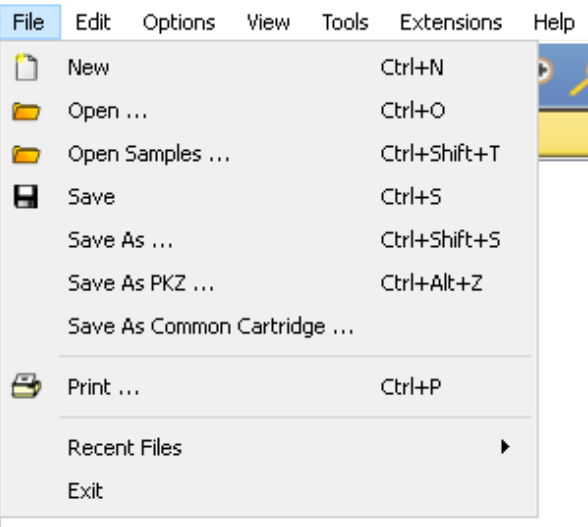
\includegraphics[scale=.35]{images/02.packet-tracer/file.png}}
    \caption{File Menù.}
\end{figure}

\subsubsection{Edit}
Il menù Edit permette di:

\begin{itemize}
    \item copiare dal progetto dei dispositivi di rete;
    \item incollare dentro il progetto dei dispositivi di rete;
    \item annullare l'ultima azione;
    \item eseguire l'ultima azione annullata.
\end{itemize}

\begin{figure}[htbp]
    \centerline{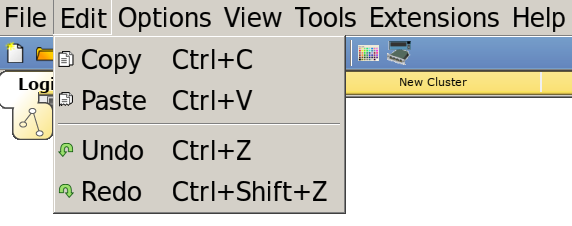
\includegraphics[scale=.35]{images/02.packet-tracer/edit.png}}
    \caption{Edit Menù.}
\end{figure}

\subsubsection{Options}
Il menù Options permette di: 

\begin{itemize}
    \item visualizzare e modificare le proprie preferenze relative al programma, come la grandezza del font;
    \item visualizzare e modificare il profilo utente corrente;
    \item visualizzare e modificare le impostazioni degli algoritmi usati;
    \item visualizzare i registri che contengono tutti i comandi eseguiti sui terminali degli apparati di rete.
\end{itemize}

\begin{figure}[htbp]
    \centerline{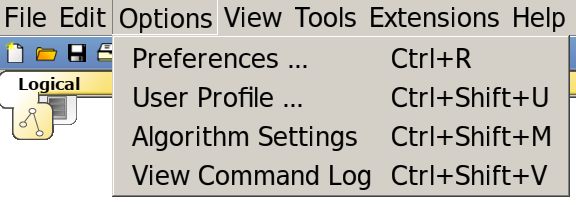
\includegraphics[scale=.35]{images/02.packet-tracer/options.png}}
    \caption{Options Menù.}
\end{figure}

\subsubsection{View}
Il menù View permette di: 

\begin{itemize}
    \item aumentare o diminuire il livello di zoom;
    \item ripristinare il livello di zoom al valore predefinito;
    \item selezionare le toolbar attive e visibili.
\end{itemize}

\begin{figure}[htbp]
    \centerline{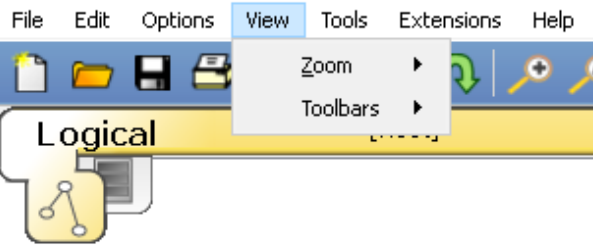
\includegraphics[scale=.35]{images/02.packet-tracer/view.png}}
    \caption{View Menù.}
\end{figure}

\subsubsection{Tools}
Il menù Tools permette di: 

\begin{itemize}
    \item disegnare delle figure e linee colorate;
    \item creare dei template per la creazione di dispositivi personalizzati.
\end{itemize}

\begin{figure}[htbp]
    \centerline{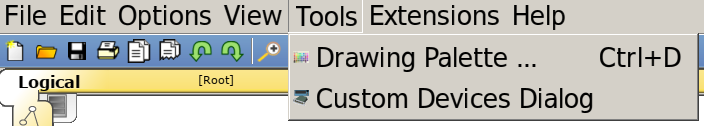
\includegraphics[scale=.3]{images/02.packet-tracer/tools.png}}
    \caption{Tools Menù.}
\end{figure}

\subsubsection{Extensions}
Il menù Extensions permette di visualizzare tutte le impostazioni relative alle estensioni installate, l'unica estensione installata in modo predefinito è quella per la progettazione Multiuser, necessaria per coinvolgere più utenti contemporaneamente nello stesso progetto.

\begin{figure}[htbp]
    \centerline{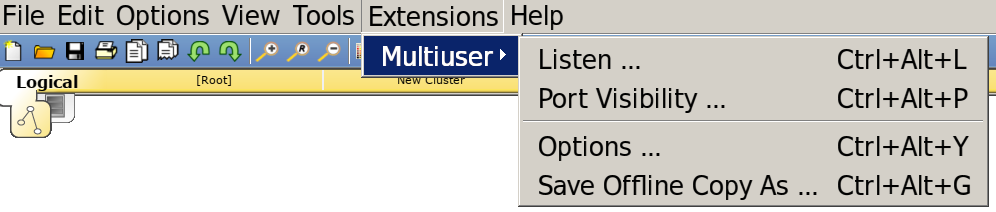
\includegraphics[scale=.35]{images/02.packet-tracer/extensions.png}}
    \caption{Extensions Menù.}
\end{figure}

\subsubsection{Help}
Il menù Help permette di: 

\begin{itemize}
    \item visualizzare la guida dedicata al programma;
    \item visualizzare tutti i tutorial disponibili;
    \item segnalare un problema all'azienda produttrice del software Cisco Systems;
    \item visualizzare le informazioni relative alla versione installata di Cisco Packet Tracer.
\end{itemize}

\begin{figure}[htbp]
    \centerline{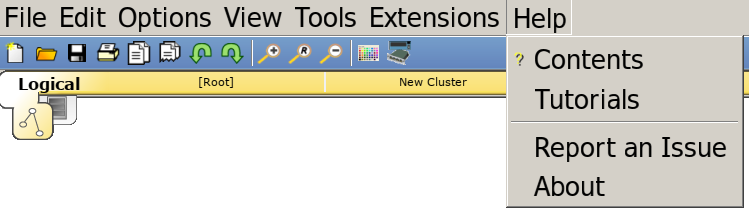
\includegraphics[scale=.3]{images/02.packet-tracer/help.png}}
    \caption{Help Menù.}
\end{figure}

\subsection{Toolbar}

\subsubsection{Toolbar Principale}
La toolbar principale posizionata in alto permette di:

\begin{itemize}
    \item creare un nuovo file partendo da zero;
    \item aprire un file già esistente;
    \item salvare le modifiche sul file corrente;
    \item stampare il progetto seconda una delle rappresentazioni disponibili;
    \item copiare dal progetto dei dispositivi di rete;
    \item incollare dentro il progetto dei dispositivi di rete;
    \item annullare l'ultima azione;
    \item eseguire l'ultima azione annullata;
    \item aumentare o diminuire il livello di zoom;
    \item ripristinare il livello di zoom al valore predefinito;
    \item disegnare delle figure e linee colorate;
    \item creare dei template per la creazione di dispositivi personalizzati;
    \item modificare la descrizione del progetto;
    \item visualizzare la guida dedicata al programma.
\end{itemize}

\begin{figure}[htbp]
    \centerline{
\includegraphics[scale=.5]{images/02.packet-tracer/top.png}}
    \caption{Toolbar Principale.}
\end{figure}

\subsubsection{Toolbar Secondaria}
La toolbar secondaria posizionata in basso permette di:

\begin{itemize}
    \item aggiungere dispositivi ed apparati di rete;
    \item visualizzare gli scenari di simulazione creati;
    \item visualizzare la tabella contenente tutti gli eventi come l'invio di un messaggio ICMP.
\end{itemize}

\begin{figure}[htbp]
    \centerline{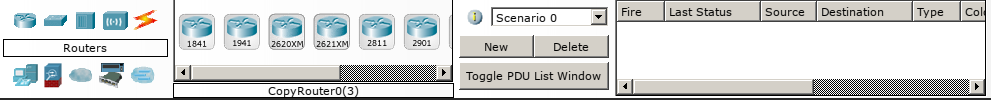
\includegraphics[scale=.17]{images/02.packet-tracer/bottom.png}}
    \caption{Toolbar Secondaria.}
\end{figure}

\subsubsection{Toolbar di Destra}
\begin{minipage}{0.85\textwidth}
    La toolbar di destra permette di:
    \begin{itemize}
        \item selezionare di uno o più dispositivi;
        \item aggiungere note e appunti alla topologia;
        \item eliminare uno o più dispositivi e connessioni;
        \item ispezionare un dispositivo;
        \item disegnare delle figure e linee colorate;
        \item cambiare la dimensione dei dispositivi;
        \item eseguire un ping semplice tra due dispositivi;
        \item eseguire un ping avanzato.
    \end{itemize}
\end{minipage}%
%
\begin{minipage}{0.15\textwidth}
    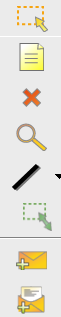
\includegraphics[width=0.7\linewidth]{images/02.packet-tracer/right.png}
\end{minipage}

\subsubsection{Logical e Physical}
Sono disponibili due modalità d'esplorazione per la progettazione: Logical e Physical; entrambe sono selezionabili cliccando sulle relative icone in alto a sinistra. La modalità Logical, l'unica usata in questa guida, permette di visualizzare la topologia di rete e i dispositivi di rete che ne fanno parte, la modalità Physical, invece, permette di visualizzare dove i dispositivi di rete sono collocati fisicamente.

\begin{figure}[htbp]
    \centerline{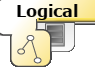
\includegraphics[scale=.6]{images/02.packet-tracer/logical_physical.png}}
    \caption{Logical e Physical.}
\end{figure}

\subsubsection{Realtime e Simulation}
Sono disponibili due modalità operative per la progettazione: Realtime e Simulation; entrambe sono selezionabili cliccando sulle relative icone in basso a destra. La modalità Realtime, quella in cui si è normalmente durante la progettazione, permette di operare in tempo reale senza poter controllare il flussi dei dati. In questa modalità sulla sinistra è anche presente il pulsante "Fast Forward Time" che permette di velocizzare le attese come quelle per l'accensione dei dispositivi. La modalità Simulation, invece, permette di filtrare il flusso dei dati e controllarlo a piacimento con comandi come Back (Indietro), Play (Esegui) e Forward (Avanti), viene generalmente usato per verificare il corretto funzionamento della rete. 

\begin{figure}[htbp]
    \centerline{
\includegraphics[scale=.5]{images/02.packet-tracer/realtime_simulation.png}}
    \caption{Realtime e Simulation.}
\end{figure}

\subsection{Opzioni Consigliate}
Al primo avvio del programma si consiglia di aprire il menu “Options”, cliccare su “Preferences” e spuntare la voce “Always Show Port Labels” (in italiano "Mostra sempre le etichette delle porte") nel caso non sia già spuntata. Questa opzione è molto utile in quanto è comune lavorare con porte specifiche degli apparati di rete e questa opzione ci permette di visualizzarne le etichette identificative nella modalità Logical rendendo la progettazione più veloce.

\smallskip

\noindent Nel caso in cui si stia utilizzando un monitor ad alta risoluzione è consigliabile aumentare la dimensione del font visualizzato accendendo alla pagina "Font" contenuta nel menu "Options". La grandezza predefinita del font è di 8 punti, con monitor di risoluzione FullHD o superiore è una buona pratica aumentare la grandezza di 2 o più punti.

\subsection{Apparati di Rete Utilizzati}

\subsubsection{Router}
Il router è un apparato di rete che permette a più dispositivi di comunicare tra loro all'interno della stessa rete informatica. Un router è dunque in grado di gestire tutti quei protocolli necessari alla creazione e gestione di una rete informatica, garantendo che tutti i dispositivi connessi comunichino efficacemente tra loro. Il router si occupa quindi di instradare i pacchetti dati in una rete tenendo conto delle regole poste dal sistemista. Nella maggior parte dei casi i router lavorano al livello 3 Rete della pila ISO/OSI.

\smallskip

\noindent In questa guida verranno usati i seguenti router:

\begin{itemize}
    \item Router Generico, può essere usato nella maggior parte dei casi, include una porta console, una porta ausiliaria, quattro porte FastEthernet (due per cavi in rame e due per cavi in fibra ottica) e due porte seriali;
    \item Router Cisco 2911, supporta il protocollo IPv6, include una porta console, una porta ausiliaria e tre porte GigabitEthernet (10 volte più veloci delle porte FastEthernet);
    \item Router Cisco WRT300N, supporta le connessioni wireless, include una porta Internet da collegare alla rete e 4 porte Ethernet per l'utilizzo interno alla sottorete.
\end{itemize}

\begin{figure}[htbp]
    \centerline{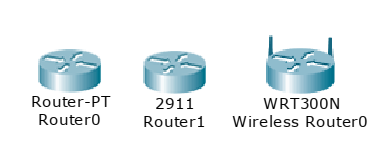
\includegraphics[scale=.5]{images/02.packet-tracer/router.png}}
    \caption{I tre router su Cisco Packet Tracer.}
\end{figure}

\subsubsection{Switch}
Uno switch è un apparato di rete che collega dei dispositivi all'interno di una rete informatica. Viene usato frequentemente nelle reti in quanto è la soluzione più economica e semplice per espandere una rete garantendo l'accesso diretto a più dispositivi. Nella maggior parte dei casi gli switch lavorano nel livello 2 Collegamento della pila ISO/OSI.

\smallskip

\noindent In questa guida verranno usati i seguenti switch:

\begin{itemize}
    \item Switch Generico, può essere usato nella maggior parte dei casi, include una porta console e sei porte FastEthernet (quattro per cavi in rame e due per cavi in fibra);
    \item Switch Cisco 2950-24, ha la peculiarità di avere una porta console e ben ventiquattro porte FastEthernet per cavi in rame.
\end{itemize}

\begin{figure}[htbp]
    \centerline{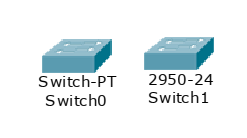
\includegraphics[scale=.5]{images/02.packet-tracer/switch.png}}
    \caption{I due switch su Cisco Packet Tracer.}
\end{figure}

\subsection{Cavi Utilizzati}
Per collegare i dispositivi tra loro e permettere la comunicazione vengono usati dei cavi, questi variano a seconda dei dispositivi che collegano, della distanza che coprono e del tipo di comunicazione scelta.

\smallskip

\noindent In questa guida verranno usati i seguenti cavi:

\begin{itemize}
    \item Cavo Ethernet dritto in rame, è il cavo più comune ed economico, viene generalmente usato per collegare i dispositivi come PC o laptop agli apparati di rete come switch e router;
    \item Cavo Ethernet incrociato in rame, è costruito con gli stessi materiali del cavo precedente ma ha la differenza che può essere solo usato per connettere tra loro due dispositivi sullo stesso livello ISO/OSI, ad esempio due Router o due Switch;
    \item Cavo in fibra ottica, è il cavo con la più grande larghezza di banda disponibile, viene generalmente usato nelle dorsali (backbone) per collegare le reti tra loro garantendo una comunicazione stabile anche quando sono molte le informazioni scambiate;
    \item Cavo Console, viene usato per accedere alla console di apparati di rete come switch e router usando PC o laptop.
\end{itemize}

\begin{figure}[htbp]
    \centering
    
\includegraphics[scale=.4]{images/02.packet-tracer/cavi.png}
    \caption{Tutti i cavi disponibili su Cisco Packet Tracer.}
\end{figure}

\subsection{Utilizzo Comune}

\subsubsection{Modifica dei moduli dei dispositivi}
Per aggiungere o rimuovere uno o più moduli è necessario spegnere il dispositivo tramite l'interruttore, si può poi rimuovere un modulo trascinandolo dal dispositivo alla colonna di sinistra contenente tutti i moduli disponibili, per aggiungerne uno invece bisogna trascinarlo dalla colonna sinistra all'apposito slot vuoto del dispositivo. Concluse le modifiche è necessario accendere il dispositivo tramite lo stesso interruttore con la quale è stato spento.

\subsubsection{Modificare il nome e l'hostname di un apparato}
Ogni apparato di rete ha un display name, nome visualizzato nella modalità Logical, e un hostname, nome associato all'apparato di rete. Questi possono essere modificati dall'interfaccia Config nella sezione Global Settings. Il display name può essere modificato anche cliccandovi sopra nella modalità Logical. L'hostname può invece essere modificato anche inserendo il seguente comando nel relativo apparato di rete.

\begin{cmds}[Router]{Configuration mode}{cmd:set-hostname}{Come cambiare l'hostname del dispositivo nel \textcolor{Highlight1}{nome specificato}}
    \$ hostname \textcolor{Highlight1}{nome}
\end{cmds}

\subsubsection{Configurazione degli indirizzi IP statici}
Per identificare le interfacce associate ai dispositivi di rete vengono utilizzati gli indirizzi IP. Il seguente comando permette di assegnare un indirizzo IPv4 statico ad un'interfaccia.

\begin{cmds}[Interface]{Configuration mode}{cmd:change-ip}{
    Configurare l'indirizzo IP di un'interfaccia con l'\textcolor{Highlight1}{indirizzo dell'interfaccia} e la \textcolor{Highlight2}{subnet della rete}.
}
    \$ ip address \textcolor{Highlight1}{192.168.0.1} \textcolor{Highlight2}{255.255.255.0}
\end{cmds}

\begin{cmds}[Interface IPv6]{Configuration mode}{cmd:change-ipv6}{Assegnare un indirizzo IPv6 statico}
    \$ ipv6 address \textcolor{Highlight1}{2001::1}/\textcolor{Highlight3}{64} % TODO?: [linklocal]
\end{cmds}

Alternativamente, gli indirizzi IP possono essere assegnati attraverso l'interfaccia Config del relativo dispositivo di rete. 

\subsubsection{Accendere le porte}
Normalmente le porte degli apparati di rete non sono accese e pronte al funzionamento, per accendere una porta è quindi necessario inserire il seguente comando.

\begin{cmds}[Interface]{Configuration mode}{cmd:no-shutdown}{Accendere un'interfaccia di rete}
    \$ no shutdown
\end{cmds}

\subsubsection{Disattivare i dns lookups}
Normalmente quando viene inserito un comando sconosciuto tramite l'interfaccia CLI nella configurazione di un apparato di rete quest'ultimo proverà a cercare un indirizzo IP con dominio corrispondente al comando sconosciuto, per fare ciò impiega più di 30 secondi che possono essere ridotti solo cancellando il comando premendo CTRL+6. Si può ovviare a questa inconvenienza inserendo il seguente comando nel relativo apparato di rete in modo da disattivare la ricerca automatica dei domini. 

\begin{cmds}{Configuration mode}{cmd:disable-dns-lookup}{Disattivare i lookup DNS}
    \$ no ip domain-lookup
\end{cmds}

\subsubsection{Salvare le modifiche fatte ad un apparato}
Dopo aver completato la configurazione dell'apparato di rete è necessario salvarla in modo che persista anche dopo lo spegnimento di quest'ultimo, ciò può essere compiuto inserendo il seguente comando.  

\begin{cmds}{Privileged mode}{cmd:save-configuration}{Salvare la configurazione del router}
    \$ copy running-config startup-config %TODO: write e' un alias. Forse e' meglio?
\end{cmds}
